% -*- coding: utf-8 -*-

\newcommand{\commentaire}[1]{}

\entete{Travaux dirigés 1 : Assembleur, affectation en C, if else.}

\vspace{-1cm}
\section{Langage machine}

L'objectif de cette première partie est de vous familiariser avec le cycle d'exécution
d'un processeur et avec la notion de flux d'instructions. Pour cela,
il vous est demandé d'écrire de petits programmes dans le langage
assembleur \C{amil} (\emph{assembleur miniature pour l'informatique de
  licence}) et de simuler leur exécution soit à la main en écrivant une trace soit en utilisant le
simulateur en ligne : \url{http://www-lipn.univ-paris13.fr/~boudes/amilweb/}.

\begin{correction}
 \paragraph{Note aux chargés de TD.}
  \begin{itemize}
  \item Dans le texte des corrections se trouvent également quelques
    explications de correction. Bien entendu, vous n'avez pas à en
    parler aux étudiants (boucle for, \C{gcc -S}, etc.).
  \item Amil est très rudimentaire dans ses possibilités d'écrire des
    commentaires. Dans cette feuille, il y a des commentaires ligne à
    ligne, mais aussi une tentative d'indiquer où sont les différents
    blocs de code dans un style balise xml/html : une ligne avec en
    commentaire \C{<bloc1>} signale la première ligne du bloc
    \C{bloc1}, une ligne avec en commentaire \C{</bloc1>} signale la
    dernière ligne du bloc, et une ligne avec en commentaire
    \C{<bloc1/>} signale l'unique ligne du bloc \C{bloc1}.
  \item les traces contiennent une colonne \emph{instructions} : cette
    colonne n'a pas lieu d'être dans les corrections (elle aide juste
    à relire la trace, qui est générée automatiquement).
  \end{itemize}
\end{correction}

\subsection*{Jeu d'instructions (simplifié)}
\begin{tabular}[c]{lp{11.3cm}}
  \C{stop} & Arrête l'exécution du programme.\\
  \C{noop} & N'effectue aucune opération.\\
  \C{saut i} & Met le compteur de programme à la valeur $i$.\\
  \C{sautpos ri j} & Si la valeur contenue dans le registre $i$ est positive ou nulle, met le compteur de programme à la valeur $j$.\\
  \C{valeur x ri} & Initialise le registre $i$ avec la valeur $x$.\\
  \C{lecture i rj} & Charge, dans le registre $j$, le contenu de la mémoire d'adresse $i$.\\
  \C{ecriture ri j} & Écrit le contenu du registre $i$ dans la mémoire d'adresse $j$.\\
  \C{inverse ri} & Inverse le signe du contenu du registre $i$.\\
  \C{add ri rj} & Ajoute la valeur du registre $i$ à celle du registre $j$ (la somme obtenue est placée dans le registre $j$).\\
  \C{soustr ri rj} & Soustrait la valeur du registre $i$ à celle du registre $j$ (la différence obtenue est placée dans le registre $j$).\\
  \C{mult ri rj} & Multiplie par la valeur du registre $i$ celle du registre $j$ (le produit obtenu est placé dans le registre $j$).%\\
  % \C{div ri rj} & Divise par la valeur du registre $i$ celle du registre $j$ (le quotient obtenu, arrondi à la valeur entière inférieure, est placé dans le registre $j$).\\
  % \multicolumn{2}{l}{\textbf{Instructions plus avancées}}\\
  % \C{et ri rj} & Effectue le et bit à bit de la valeur du registre $i$ et de celle du registre $j$. Le résultat est placé dans le registre $j$.\\
  % \C{lecture *ri rj} & Charge, dans le registre $j$, le contenu de la mémoire dont l'adresse est la valeur du registre $i$\\
  % \C{ecriture ri *rj} & Écrit le contenu du registre $i$ dans la mémoire dont  l'adresse est la valeur du registre $j$.
\end{tabular}

\noindent

\subsection{Écriture de programmes simples}
Écrire les programmes répondant aux problèmes suivants :
\begin{enumerate}
\item Soit la valeur 8 contenue dans la case mémoire d'adresse 10. Recopier cette valeur à l'adresse 11.
  \begin{correction}%OK
    \begin{listing}{1}
      lecture 10 r0
      ecriture r0 11
      stop
    \end{listing}

\begin{figure} %\begin{sidewaysfigure} ...
  \centering
% bin/amiltrace examples/max2td.ail traces_latex/max2td.tex
  \begin{tabular}[c]{|c|c|c|c|c|c|}
\hline
Cycles & CP & instruction & r0& 10& 11\\ \hline
INIT & 1 & & ? & 5
 & ?
 \\ \hline1 & 2 & \commentaire{Lecture de la donnée d'adresse 10 dans le registre 0
} lecture 10 r0
 & 5 & & \\ \hline
2 & 3 & \commentaire{Écriture du registre 0 à l'adresse 11
} ecriture r0 11
 & & & 5
 \\ \hline
3 & 4 & \commentaire{Fin du processus.
} stop
 & & & \\ \hline
\end{tabular}
  \caption{Simulation de la copie de valeur}
  \label{trace_copie_val}
\end{figure}
  \end{correction}
\item Soit une valeur quelconque, $a$, contenue à l'adresse 10. Écrire
  la valeur de $a \times 2 + 1$ dans  la case d'adresse 11.
  \begin{correction}%OK
    \begin{listing}{1}
      lecture 10 r0
      valeur 2 r1
      mult r1 r0
      valeur 1 r1
      add r1 r0
      ecriture r0 11
      stop
    \end{listing}
  \end{correction}
\end{enumerate}

\subsection{Trace de programme assembleur}
Nous allons désormais produire une représentation de l'exécution pas à pas de nos programmes. Une \emph{trace} d'un programme assembleur sera un tableau dont chaque ligne correspond à l'exécution d'une instruction par le processeur.  Une colonne contiendra le cycle d'horloge du processeur et une autre colonne le compteur de programme. Il y aura également une colonne par registre utilisé dans le programme et par case mémoire où des données sont lues ou écrites par les instructions du programme. Une première ligne, d'initialisation, montrera l'état de ces registres et cases mémoires avant le début du programme. Ensuite, chaque exécution d'instruction sera représentée par une nouvelle ligne du tableau, jusqu'à exécution de l'instruction \C{stop}. Dans cette ligne nous représenterons le cycle d'horloge du processeur (en commençant à 0 pour la ligne d'initialisation),  la valeur du compteur de programme après exécution de l'instruction, et, s'il y a lieu, la valeur du registre ou de la case mémoire modifiée par le programme. 

\subsubsection{Exemple de trace et première trace}


\begin{minipage}[t]{0.35\linewidth}
Soit le programme ci-dessous :

\listinginput{1}{progs/exempletrace.ail}
\end{minipage}\hfill
\begin{minipage}[t]{0.6\linewidth}
On représentera alors sa trace comme ceci : 
\bigskip

\begin{tabular}[c]{l||c|c|c|c|c|c|}
\hline
 \emph{Instructions} & Cycles & CP& r0& r2& 10& 11\\ \hline
\hfill Initialisation & 0 & 1 & ? & ? & 14
 & ?
 \\ \hline \commentaire{Lecture de la donnée d'adresse 10 dans le registre 0
} \C{lecture 10 r0
} & 1 & 2  & 14 & & &\\ \hline
 \commentaire{Initialisation du registre 2 à 5
} \C{valeur 5 r2
} & 2 & 3  & & 5 & &\\ \hline
 \commentaire{Soustrait la valeur du registre 2 au registre 0
} \C{soustr r2 r0
} & 3 & 4  & 9 & & &\\ \hline
 \commentaire{Si la valeur (9) du registre 0 est positive, saute à l'adresse 8
} \C{sautpos r0 8
} & 4 & \textbf{8} & & & &\\ \hline
 \commentaire{Écriture du registre 0 à l'adresse 11
} \C{ecriture r0 11
} & 5 & 9  & & & & 9
\\ \hline
 \commentaire{Fin du processus.
} \C{stop
} & 6 & 10  & & & &\\ \hline
\end{tabular}
\end{minipage}
\medskip

La colonne \emph{Instructions} n'est pas nécessaire, elle sert juste ici à la compréhension, sans cette colonne le mot-clé \emph{initialisation} pourra être placé dans la colonne \emph{Cycles}. Remarquez par exemple qu'il n'y a pas de colonne pour le registre 1, puisque celui-ci n'est pas utilisé.


\begin{enumerate}
\item Refaire la trace du programme où la valeur 14 à l'adresse 10 est remplacée
  par 2.

\item  Quelles sont les valeurs contenues dans les registres 0, 1 et 2
  après arrêt sur \C{stop} ?
\end{enumerate}
\begin{correction}
  \input{progs/exempletraceAlt.tex}

La valeur contenue dans le registre 0 est 0, celle contenue dans le registre 1 est indéterminée, celle contenue dans le registre 2 est 5.
\end{correction}

\subsection{Exécution conditionnelle d'instructions}

À l'aide de l'instruction \verb|sautpos|, écrire les programmes correspondant aux
algorithmes suivants et les exécuter sur un exemple (trace ou simulateur) afin de tester leur correction :
\begin{enumerate}
\item Soient la valeur $a$ à l'adresse 15, $b$ à l'adresse 16. Si $a >= b$ alors écrire $a$ à l'adresse 17 sinon écrire $b$ à l'adresse 17.
\begin{correction}
    \listinginput{1}{progs/max2td.ail}
\begin{figure} %\begin{sidewaysfigure} ...
  \centering
 \begin{tabular}[c]{l||c|c|c|c|c|c|c|}
\hline
 \emph{Instructions} & Cycles & CP& r0& r1& 15& 16& 17\\ \hline
\hfill Initialisation & 0 & 1 & ? & ? & 23
 & 45
 & ?
 \\ \hline \commentaire{Lecture de la donnée d'adresse 15 dans le registre 0
} \C{lecture 15 r0
} & 1 & 2  & 23 & & & &\\ \hline
 \commentaire{Lecture de la donnée d'adresse 16 dans le registre 1
} \C{lecture 16 r1
} & 2 & 3  & & 45 & & &\\ \hline
 \commentaire{Soustrait la valeur du registre 1 au registre 0
} \C{soustr r1 r0
} & 3 & 4  & -22 & & & &\\ \hline
 \commentaire{Si la valeur (-22) du registre 0 est positive, saute à l'adresse 8
} \C{sautpos r0 8
} & 4 & 5  & & & & &\\ \hline
 \commentaire{Lecture de la donnée d'adresse 16 dans le registre 0
} \C{lecture 16 r0
} & 5 & 6  & 45 & & & &\\ \hline
 \commentaire{Écriture du registre 0 à l'adresse 17
} \C{ecriture r0 17
} & 6 & 7  & & & & & 45
\\ \hline
 \commentaire{Saut à l'adresse 10
} \C{saut 10
} & 7 & \textbf{10} & & & & &\\ \hline
 \commentaire{Fin du processus.
} \C{stop
} & 8 & 11  & & & & &\\ \hline
\end{tabular}
  \caption{Simulation du calcul du max de a et b (1)}
  \label{simmax1}
\end{figure}
\begin{figure}
  \centering
  \begin{tabular}[c]{|c|c|c|c|c|c|c|c|}
\hline
Cycles & CP & instruction & r0& r1& 15& 16& 17\\ \hline
INIT & 1 & & ? & ? & 45
 & 23
 & ?
 \\ \hline1 & 2 & \commentaire{Lecture de la donnée d'adresse 15 dans le registre 0
} lecture 15 r0
 & 45 & & & & \\ \hline
2 & 3 & \commentaire{Lecture de la donnée d'adresse 16 dans le registre 1
} lecture 16 r1
 & & 23 & & & \\ \hline
3 & 4 & \commentaire{Inversion du signe de la valeur du registre 1
} inverse r1
 & & -23 & & & \\ \hline
4 & 5 & \commentaire{Ajout de la valeur du registre 0 au registre 1
} add r0 r1
 & & 22 & & & \\ \hline
5 &\textbf{9} & \commentaire{Si la valeur (22) du registre 1 est positive, saute a l'adresse 9
} sautpos r1 9
 & & & & & \\ \hline
6 & 10 & \commentaire{Lecture de la donnée d'adresse 15 dans le registre 0
} lecture 15 r0
 & 45 & & & & \\ \hline
7 & 11 & \commentaire{Écriture du registre 0 à l'adresse 17
} ecriture r0 17
 & & & & & 45
 \\ \hline
8 & 12 & \commentaire{Fin du processus.
} stop
 & & & & & \\ \hline
\end{tabular}
  \caption{Simulation du calcul du max de a et b (2)}
  \label{simmax2}
\end{figure}
\end{correction}
% \item Soient la valeur $a$ à l'adresse 1, $b$ à l'adresse 2. Si $a < b$ alors écrire $a$ à l'adresse 3 sinon écrire $b$ à l'adresse 3$.
\item Soit l'âge d'une personne à l'adresse 15. Si cette personne est majeure alors écrire $1$ à l'adresse 16 sinon écrire $0$ à l'adresse 16.
 \begin{correction}
\listinginput{1}{../mini-assembleur/examples/majeur.ail}
\begin{figure}
  \centering
  \begin{tabular}[c]{|c|c|c|c|c|c|c|}
\hline
Cycles & CP & instruction & r0& r1& 15& 16\\ \hline
INIT & 1 & & ? & ? & 17
 & ?
 \\ \hline1 & 2 & \commentaire{Lecture de la donnée d'adresse 15 dans le registre 0
} lecture 15 r0
 & 17 & & & \\ \hline
2 & 3 & \commentaire{Initialisation du registre 1 à -18
} valeur -18 r1
 & & -18 & & \\ \hline
3 & 4 & \commentaire{Ajout de la valeur du registre 0 au registre 1
} add r0 r1
 & & -1 & & \\ \hline
4 & 5 & \commentaire{Si la valeur (-1) du registre 1 est positive, saute a l'adresse 8
} sautpos r1 8
 & & & & \\ \hline
5 & 6 & \commentaire{Initialisation du registre 0 à 0
} valeur 0 r0
 & 0 & & & \\ \hline
6 & 7 & \commentaire{Écriture du registre 0 à l'adresse 16
} ecriture r0 16
 & & & & 0
 \\ \hline
7 &\textbf{10} & \commentaire{Saut a l'adresse 10
} saut 10
 & & & & \\ \hline
8 & 11 & \commentaire{Fin du processus.
} stop
 & & & & \\ \hline
\end{tabular}
  \caption{Simulation du test de la majorité (1)}
  \label{simmaj1}
\end{figure}
\begin{figure}
  \centering
  \begin{tabular}[c]{|c|c|c|c|c|c|c|}
\hline
Cycles & CP & instruction & r0& r1& 15& 16\\ \hline
INIT & 1 & & ? & ? & 20
 & ?
 \\ \hline1 & 2 & \commentaire{Lecture de la donnée d'adresse 15 dans le registre 0
} lecture 15 r0
 & 20 & & & \\ \hline
2 & 3 & \commentaire{Initialisation du registre 1 à -18
} valeur -18 r1
 & & -18 & & \\ \hline
3 & 4 & \commentaire{Ajout de la valeur du registre 0 au registre 1
} add r0 r1
 & & 2 & & \\ \hline
4 &\textbf{8} & \commentaire{Si la valeur (2) du registre 1 est positive, saute a l'adresse 8
} sautpos r1 8
 & & & & \\ \hline
5 & 9 & \commentaire{Initialisation du registre 0 à 1
} valeur 1 r0
 & 1 & & & \\ \hline
6 & 10 & \commentaire{Écriture du registre 0 à l'adresse 16
} ecriture r0 16
 & & & & 1
 \\ \hline
7 & 11 & \commentaire{Fin du processus.
} stop
 & & & & \\ \hline
\end{tabular}
  \caption{Simulation du test de la majorité (2)}
  \label{simmaj2}
\end{figure}
 \end{correction}
\item Soient trois cases mémoires contenant trois entiers, $a$, $b$ et $c$. Calculer le
  minimum de ces trois entiers et l'écrire dans une autre case
  mémoire. \emph{Commencer par réflechir à l'algorithme.}
\begin{correction}
\begin{itemize}
\item Soient $a$, $b$ et $c$ trois entiers
\begin{listing}{20}
12 # a    
23 # b
6  # c
?  # min
\end{listing}
\item $\text{min}$ est initialise à $a$ (par défaut)
\begin{listing}{1}
lecture 20 r0
ecriture r0 23
\end{listing}
\item Si $b < \text{min}$ alors $\text{min}$ vaut $b$
\begin{listing}{3}
lecture 21 r0
lecture 23 r1
inverse r1
add r0 r1    # r1 vaut b - min
sautpos r1 9 
ecriture r0 23
\end{listing}
\item Si $c < \text{min}$ alors $\text{min}$ vaut $c$
\begin{listing}{9}
lecture 22 r0
lecture 23 r1
inverse r1
add r0 r1 # r1 vaut c - min
sautpos r1 15
ecriture r0 23
\end{listing}
\item $\text{min}$ contient le minimum de $a$, $b$ et $c$ 
\begin{listing}{15}
stop
\end{listing}
\end{itemize}
\end{correction}
\end{enumerate}

% Soit la donnée $x$ d'adresse $15$. On veut écrire la valeur absolue de $x$ à
%   l'adresse $16$.
% \begin{enumerate}
% \item Décrire un algorithme réalisant cette tâche.
%   \begin{correction}
%     \begin{itemize}
%     \item Si $x < 0$
%     \item Alors écrire $-x$ à l'adresse $16$
%      \item Sinon écrire $x$ à l'adresse $16$
% % =======
% %     \item Si $x \geq 0$
% %     \item Alors écrire $x$ à l'adresse $16$
% %      \item Sinon écrire $-x$ à l'adresse $16$
% % >>>>>>> .r117
%     \end{itemize}
% \end{correction}
% \item Écrire un programme réalisant cette tâche.
% \begin{correction}
% \begin{itemize}
% \item Si $x < 0$
% \begin{listing}{1}
% lecture 15 r0    
% sautpos r0 6    <-- saute sur le sinon
% \end{listing}
% \item Alors écrire $-x$ à l'adresse $16$
% \begin{listing}{3}
% inverse r0
% ecriture r0 16
% saut 7         <-- saute sur le stop
% \end{listing}
% \item Sinon écrire $x$ à l'adresse $16$
% \begin{listing}{6}
% ecriture r0 16
% \end{listing}
% \item suite du programme
% \begin{listing}{7}
% stop
% ?
% \end{listing}
% \vdots
% \begin{listing}{14}
% ?
% 5
% ?
% \end{listing}
% \end{itemize}
% \end{correction}

% \item Construire une trace de votre programme lorsque $x$ vaut $5$,
%   puis lorsque $x$ vaut $-5$.
% \end{enumerate}

% \begin{correction}
% Voir les figures~\ref{fig:abspos} et~\ref{fig:absposmoins}.
%   \begin{figure}[tbp]
%     \centering
%     \begin{tabular}[c]{l||c|c|c|c|c|}
\hline
 \emph{Instructions} & Cycles & CP& r0& 15& 16\\ \hline
\hfill Initialisation & 0 & 1 & ? & 5
 & ?
 \\ \hline \commentaire{Lecture de la donnée d'adresse 15 dans le registre 0
} \C{lecture 15 r0
} & 1 & 2  & 5 & &\\ \hline
 \commentaire{Si la valeur (5) du registre 0 est positive, saute à l'adresse 6
} \C{sautpos r0 6
} & 2 & \textbf{6} & & &\\ \hline
 \commentaire{Écriture du registre 0 à l'adresse 16
} \C{ecriture r0 16
} & 3 & 7  & & & 5
\\ \hline
 \commentaire{Fin du processus.
} \C{stop
} & 4 & 8  & & &\\ \hline
\end{tabular}
%     \caption{Trace du calcul de la valeur absolue de $5$}
%     \label{fig:abspos}
%   \end{figure}
%   \begin{figure}[tbp]
%     \centering
%     \begin{tabular}[c]{l||c|c|c|c|c|}
\hline
 \emph{Instructions} & Cycles & CP& r0& 15& 16\\ \hline
\hfill Initialisation & 0 & 1 & ? & -5
 & ?
 \\ \hline \commentaire{Lecture de la donnée d'adresse 15 dans le registre 0
} \C{lecture 15 r0
} & 1 & 2  & -5 & &\\ \hline
 \commentaire{Si la valeur (-5) du registre 0 est positive, saute à l'adresse 6
} \C{sautpos r0 6
} & 2 & 3  & & &\\ \hline
 \commentaire{Inversion du signe de la valeur du registre 0
} \C{inverse r0
} & 3 & 4  & 5 & &\\ \hline
 \commentaire{Écriture du registre 0 à l'adresse 16
} \C{ecriture r0 16
} & 4 & 5  & & & 5
\\ \hline
 \commentaire{Saut à l'adresse 7
} \C{saut 7
} & 5 & \textbf{7} & & &\\ \hline
 \commentaire{Fin du processus.
} \C{stop
} & 6 & 8  & & &\\ \hline
\end{tabular}
%     \caption{Trace du calcul de la valeur absolue de $-5$}
%     \label{fig:absposmoins}
%   \end{figure}
% \clearpage
% \end{correction}

\subsection{Boucles infinies}


Avec l'instruction \verb|saut|, écrire un programme qui ne
termine jamais.

\begin{correction}
\begin{listing}{1}
saut 1
stop # <- jamais atteint
\end{listing}
\end{correction}

% \item Avec l'instruction \verb|sautpos|, écrire un programme qui ne
%   termine jamais.
% \begin{correction}
% \begin{listing}{1}
% valeur 0 r0
% sautpos r0 1
% stop # <- jamais atteint
% \end{listing}  
% \end{correction}


% \subsection{Boucles de calculs itératifs}

% Soit un entier $n$ d'adresse $15$.
% \begin{enumerate}
% \item Écrire un programme qui lorsque $n \geq 0$, écrit la valeur $n$
%   à l'adresse $16$, puis, toujours à l'adresse $16$, écrit la valeur
%   $n - 1$, puis $n - 2$, et ainsi de suite jusqu'à écrire $0$, après
%   quoi le programme termine. Si $n$ est négatif, le programme ne fait
%   rien.
%   \begin{correction}
%     \begin{itemize}
%     \item $x$ vaut $n$
%     \item Tant que $x \geq 0$ : écrire $x$ puis enlever $1$ à $x$
%     \end{itemize}

%     Pour la traduction en assembleur de l'algorithme, on imite le
%     schéma de traduction standard du \C{while (...) \{ ... \}} . Dans
%     cette traduction le test décidant de (la répétition de)
%     l'exécution de la boucle, vient juste après le corps de la boucle
%     plutôt qu'avant. Et il y a juste avant le corps de boucle un saut
%     vers ce test. Ainsi la condition de saut traduit la condition
%     d'exécution (non sa négation) en un minimum de lignes.

%     \listinginput{1}{progs/decrement.ail}
%     \begin{figure}[tbp]
%       \centering
%       \begin{tabular}[c]{l||c|c|c|c|c|c|}
\hline
 \emph{Instructions} & Cycles & CP& r0& r1& 15& 16\\ \hline
\hfill Initialisation & 0 & 1 & ? & ? & 3
 & ?
 \\ \hline \commentaire{Lecture de la donnée d'adresse 15 dans le registre 0
} \C{lecture 15 r0
} & 1 & 2  & 3 & & &\\ \hline
 \commentaire{Saut à l'adresse 6
} \C{saut 6
} & 2 & \textbf{6} & & & &\\ \hline
 \commentaire{Si la valeur (3) du registre 0 est positive, saute à l'adresse 3
} \C{sautpos r0 3
} & 3 & \textbf{3} & & & &\\ \hline
 \commentaire{Écriture du registre 0 à l'adresse 16
} \C{ecriture r0 16
} & 4 & 4  & & & & 3
\\ \hline
 \commentaire{Initialisation du registre 1 à -1
} \C{valeur -1 r1
} & 5 & 5  & & -1 & &\\ \hline
 \commentaire{Ajout de la valeur du registre 1 au registre 0
} \C{add r1 r0
} & 6 & 6  & 2 & & &\\ \hline
 \commentaire{Si la valeur (2) du registre 0 est positive, saute à l'adresse 3
} \C{sautpos r0 3
} & 7 & \textbf{3} & & & &\\ \hline
 \commentaire{Écriture du registre 0 à l'adresse 16
} \C{ecriture r0 16
} & 8 & 4  & & & & 2
\\ \hline
 \commentaire{Initialisation du registre 1 à -1
} \C{valeur -1 r1
} & 9 & 5  & & -1 & &\\ \hline
 \commentaire{Ajout de la valeur du registre 1 au registre 0
} \C{add r1 r0
} & 10 & 6  & 1 & & &\\ \hline
 \commentaire{Si la valeur (1) du registre 0 est positive, saute à l'adresse 3
} \C{sautpos r0 3
} & 11 & \textbf{3} & & & &\\ \hline
 \commentaire{Écriture du registre 0 à l'adresse 16
} \C{ecriture r0 16
} & 12 & 4  & & & & 1
\\ \hline
 \commentaire{Initialisation du registre 1 à -1
} \C{valeur -1 r1
} & 13 & 5  & & -1 & &\\ \hline
 \commentaire{Ajout de la valeur du registre 1 au registre 0
} \C{add r1 r0
} & 14 & 6  & 0 & & &\\ \hline
 \commentaire{Si la valeur (0) du registre 0 est positive, saute à l'adresse 3
} \C{sautpos r0 3
} & 15 & \textbf{3} & & & &\\ \hline
 \commentaire{Écriture du registre 0 à l'adresse 16
} \C{ecriture r0 16
} & 16 & 4  & & & & 0
\\ \hline
 \commentaire{Initialisation du registre 1 à -1
} \C{valeur -1 r1
} & 17 & 5  & & -1 & &\\ \hline
 \commentaire{Ajout de la valeur du registre 1 au registre 0
} \C{add r1 r0
} & 18 & 6  & -1 & & &\\ \hline
 \commentaire{Si la valeur (-1) du registre 0 est positive, saute à l'adresse 3
} \C{sautpos r0 3
} & 19 & 7  & & & &\\ \hline
 \commentaire{Fin du processus.
} \C{stop
} & 20 & 8  & & & &\\ \hline
\end{tabular}
%       \caption{Décrément pour $n = 3$}
%       \label{fig:decr}
%     \end{figure}
%   \end{correction}
% \item Décrire un algorithme calculant la somme des entiers $0$, $1$,
%   \ldots, $n$. Par convention cette somme, $\sum^n_{i = 0} i
%   = 0 + 1 + \ldots + n$ est nulle lorsque $n < 0$. Écrire le programme
%   correspondant. Le résultat de la sommation sera écrit à l'adresse
%   $16$.
% \begin{correction}
% \textbf{Attention plusieurs réponses correctes sont possibles, mais
% il faudra donner la correction suivante.}

% La correction suivante reprend la traduction en assembleur (\C{gcc
%   -S}) d'un \C{while (...) {...}}, ou d'une boucle \C{for( i = 0; i <=
%   n; i = i + 1)} en C. L'algorithme consiste en copier la formule de
% la somme :
% \begin{itemize}
% \item la somme vaut $0$,  $i$ vaut $0$.
% \item Tant que $i \leq n$, ajouter $x_i$ à la somme puis ajouter $1$ à
%   $i$.
% \end{itemize}

% Le programme est alors :

% \listinginput{1}{progs/gauss1.ail}
% \begin{figure}[tbp]
%   \centering \begin{tabular}[c]{l||c|c|c|c|c|c|c|c|}
\hline
 \emph{Instructions} & Cycles & CP& r0& r1& r2& r3& 15& 16\\ \hline
\hfill Initialisation & 0 & 1 & ? & ? & ? & ? & 3
 & ?
 \\ \hline \commentaire{Initialisation du registre 1 à 0
} \C{valeur 0 r1
} & 1 & 2  & & 0 & & & &\\ \hline
 \commentaire{Initialisation du registre 2 à 0
} \C{valeur 0 r2
} & 2 & 3  & & & 0 & & &\\ \hline
 \commentaire{Saut à l'adresse 7
} \C{saut 7
} & 3 & \textbf{7} & & & & & &\\ \hline
 \commentaire{Lecture de la donnée d'adresse 15 dans le registre 0
} \C{lecture 15 r0
} & 4 & 8  & 3 & & & & &\\ \hline
 \commentaire{Soustrait la valeur du registre 2 au registre 0
} \C{soustr r2 r0
} & 5 & 9  & 3 & & & & &\\ \hline
 \commentaire{Si la valeur (3) du registre 0 est positive, saute à l'adresse 4
} \C{sautpos r0 4
} & 6 & \textbf{4} & & & & & &\\ \hline
 \commentaire{Ajout de la valeur du registre 2 au registre 1
} \C{add r2 r1
} & 7 & 5  & & 0 & & & &\\ \hline
 \commentaire{Initialisation du registre 3 à 1
} \C{valeur 1 r3
} & 8 & 6  & & & & 1 & &\\ \hline
 \commentaire{Ajout de la valeur du registre 3 au registre 2
} \C{add r3 r2
} & 9 & 7  & & & 1 & & &\\ \hline
 \commentaire{Lecture de la donnée d'adresse 15 dans le registre 0
} \C{lecture 15 r0
} & 10 & 8  & 3 & & & & &\\ \hline
 \commentaire{Soustrait la valeur du registre 2 au registre 0
} \C{soustr r2 r0
} & 11 & 9  & 2 & & & & &\\ \hline
 \commentaire{Si la valeur (2) du registre 0 est positive, saute à l'adresse 4
} \C{sautpos r0 4
} & 12 & \textbf{4} & & & & & &\\ \hline
 \commentaire{Ajout de la valeur du registre 2 au registre 1
} \C{add r2 r1
} & 13 & 5  & & 1 & & & &\\ \hline
 \commentaire{Initialisation du registre 3 à 1
} \C{valeur 1 r3
} & 14 & 6  & & & & 1 & &\\ \hline
 \commentaire{Ajout de la valeur du registre 3 au registre 2
} \C{add r3 r2
} & 15 & 7  & & & 2 & & &\\ \hline
 \commentaire{Lecture de la donnée d'adresse 15 dans le registre 0
} \C{lecture 15 r0
} & 16 & 8  & 3 & & & & &\\ \hline
 \commentaire{Soustrait la valeur du registre 2 au registre 0
} \C{soustr r2 r0
} & 17 & 9  & 1 & & & & &\\ \hline
 \commentaire{Si la valeur (1) du registre 0 est positive, saute à l'adresse 4
} \C{sautpos r0 4
} & 18 & \textbf{4} & & & & & &\\ \hline
 \commentaire{Ajout de la valeur du registre 2 au registre 1
} \C{add r2 r1
} & 19 & 5  & & 3 & & & &\\ \hline
 \commentaire{Initialisation du registre 3 à 1
} \C{valeur 1 r3
} & 20 & 6  & & & & 1 & &\\ \hline
 \commentaire{Ajout de la valeur du registre 3 au registre 2
} \C{add r3 r2
} & 21 & 7  & & & 3 & & &\\ \hline
 \commentaire{Lecture de la donnée d'adresse 15 dans le registre 0
} \C{lecture 15 r0
} & 22 & 8  & 3 & & & & &\\ \hline
 \commentaire{Soustrait la valeur du registre 2 au registre 0
} \C{soustr r2 r0
} & 23 & 9  & 0 & & & & &\\ \hline
 \commentaire{Si la valeur (0) du registre 0 est positive, saute à l'adresse 4
} \C{sautpos r0 4
} & 24 & \textbf{4} & & & & & &\\ \hline
 \commentaire{Ajout de la valeur du registre 2 au registre 1
} \C{add r2 r1
} & 25 & 5  & & 6 & & & &\\ \hline
 \commentaire{Initialisation du registre 3 à 1
} \C{valeur 1 r3
} & 26 & 6  & & & & 1 & &\\ \hline
 \commentaire{Ajout de la valeur du registre 3 au registre 2
} \C{add r3 r2
} & 27 & 7  & & & 4 & & &\\ \hline
 \commentaire{Lecture de la donnée d'adresse 15 dans le registre 0
} \C{lecture 15 r0
} & 28 & 8  & 3 & & & & &\\ \hline
 \commentaire{Soustrait la valeur du registre 2 au registre 0
} \C{soustr r2 r0
} & 29 & 9  & -1 & & & & &\\ \hline
 \commentaire{Si la valeur (-1) du registre 0 est positive, saute à l'adresse 4
} \C{sautpos r0 4
} & 30 & 10  & & & & & &\\ \hline
 \commentaire{Écriture du registre 1 à l'adresse 16
} \C{ecriture r1 16
} & 31 & 11  & & & & & & 6
\\ \hline
 \commentaire{Fin du processus.
} \C{stop
} & 32 & 12  & & & & & &\\ \hline
\end{tabular}
%   \caption{Somme des entiers de $0$ à $3$}
%   \label{fig:gauss1}
% \end{figure}


% La boucle incrémente $i$. Dans amil, à cause de la difficulté à écrire
% des tests tels que $i \leq n$, il serait plus rapide sur cet exercice
% de décrémenter $n$ jusqu'à $0$ comme à la question précédente :

% \begin{itemize}
% \item $x$ vaut $n$, la somme vaut $0$
% \item Tant que $x \geq 0$, ajouter $x$ à la somme et décrementer $x$.
% \end{itemize}

% Cette réponse est correcte et on peut encourager dans un premier temps
% les étudiants qui cherchent dans cette direction, mais, pour les
% préparer à la suite du cours, il faut leur donner la correction qui
% incrémente l'indice.

% Parmi les autres programmes corrects possibles, des étudiants peuvent
% même penser à la formule de Gauss $\sum^n_{i = 0} i = \frac{n (n +
%   1)}{2}$. 



% % Solution de Gauss (trace figure~\ref{fig:gauss3}).

% % \listinginput{1}{progs/gauss3.ail}
% %     \begin{figure}[tbp]
% %       \centering
% %       \begin{tabular}[c]{l||c|c|c|c|c|c|}
\hline
 \emph{Instructions} & Cycles & CP& r0& r1& 15& 16\\ \hline
\hfill Initialisation & 0 & 1 & ? & ? & 3
 & ?
 \\ \hline \commentaire{Lecture de la donnée d'adresse 15 dans le registre 0
} \C{lecture 15 r0
} & 1 & 2  & 3 & & &\\ \hline
 \commentaire{Lecture de la donnée d'adresse 15 dans le registre 1
} \C{lecture 15 r1
} & 2 & 3  & & 3 & &\\ \hline
 \commentaire{Ajout de la valeur 1 au registre 1
} \C{add 1 r1
} & 3 & 4  & & 4 & &\\ \hline
 \commentaire{Multiplie la valeur du registre 1 par celle du registre 0
} \C{mult r0 r1
} & 4 & 5  & & 12 & &\\ \hline
 \commentaire{Divise la valeur du registre 1 par 2
} \C{div 2 r1
} & 5 & 6  & & 6 & &\\ \hline
 \commentaire{Écriture du registre 1 à l'adresse 16
} \C{ecriture r1 16
} & 6 & 7  & & & & 6
\\ \hline
 \commentaire{Fin du processus.
} \C{stop
} & 7 & 8  & & & &\\ \hline
\end{tabular}
% %       \caption{Somme des entiers de $0$ à $3$ (3)}
% %       \label{fig:gauss3}
% %     \end{figure}

% \end{correction}
% \item (Optionnel) Tester votre programme en construisant sa trace pour
%   $n = 3$.

%   \begin{correction}
%     Cette question n'est à traitée qu'au cas où les étudiants auraient
%     eu de grosses difficultés avec la précédente trace. Dans un groupe
%     ou les traces passent mal, la similitude avec l'exercice
%     précédent peut aider à leur faire refaire une trace (dans ce cas
%     on donne la correction). La trace est donnée
%     figure~\ref{fig:gauss1}.
%   \end{correction}
% \end{enumerate}

% \subsection{Boucles de parcours (exercice facultatif)}

% Soient $n$ entiers $x_1$, \ldots, $x_n$ rangées aux adresses $30 + 1$,
% \ldots, $30 + n$. La valeur $n > 0$ est elle même rangée à l'adresse
% $30$.

% \begin{enumerate}
% \item Décrire un algorithme qui effectue la somme $\sum^{n}_{i = 1} x_i
%   = x_1 + \ldots + x_n$. 
% \begin{correction}
% \begin{itemize}
% \item La somme vaut $0$
% \item Pour $i$ allant de $1$ à $n$, ajouter $x_i$ à la somme.
% \end{itemize}
% \end{correction}
% \item Écrire un programme réalisant cet algorithme. (Vous aurez besoin
%   des instructions \C{lecture *ri rj} et \C{ecriture ri *rj}). Le
%   résultat sera écrit à l'adresse $30 + n + 1$.

% \begin{correction}
% \listinginput{1}{progs/bouclesomme.ail}
%     \begin{figure}[tbp]
%       \centering\small
%       \begin{tabular}[c]{l||c|c|c|c|c|c|c|c|c|c|c|c|}
\hline
 \emph{Instructions} & Cycles & CP& r0& r1& r2& r4& r5& 30& 31& 32& 33& 34\\ \hline
\hfill Initialisation & 0 & 1 & ? & ? & ? & ? & ? & 3
 & 100
 & 1
 & 10
 & ?
 \\ \hline \commentaire{Initialisation du registre 0 à 0
} \C{valeur 0 r0
} & 1 & 2  & 0 & & & & & & & & &\\ \hline
 \commentaire{Initialisation du registre 2 à 1
} \C{valeur 1 r2
} & 2 & 3  & & & 1 & & & & & & &\\ \hline
 \commentaire{Saut à l'adresse 9
} \C{saut 9
} & 3 & \textbf{9} & & & & & & & & & &\\ \hline
 \commentaire{Lecture de la donnée d'adresse 30 dans le registre 1
} \C{lecture 30 r1
} & 4 & 10  & & 3 & & & & & & & &\\ \hline
 \commentaire{Soustrait la valeur du registre 2 au registre 1
} \C{soustr r2 r1
} & 5 & 11  & & 2 & & & & & & & &\\ \hline
 \commentaire{Si la valeur (0) du registre 3 est positive, saute à l'adresse 4
} \C{sautpos r3 4
} & 6 & \textbf{4} & & & & & & & & & &\\ \hline
 \commentaire{Initialisation du registre 4 à 30
} \C{valeur 30 r4
} & 7 & 5  & & & & 30 & & & & & &\\ \hline
 \commentaire{Ajout de la valeur du registre 2 au registre 4
} \C{add r2 r4
} & 8 & 6  & & & & 31 & & & & & &\\ \hline
 \commentaire{Lecture de la donnée d'adresse 31 dans le registre 5
} \C{lecture *r4 r5
} & 9 & 7  & & & & & 100 & & & & &\\ \hline
 \commentaire{Ajout de la valeur du registre 5 au registre 0
} \C{add r5 r0
} & 10 & 8  & 100 & & & & & & & & &\\ \hline
 \commentaire{Ajout de la valeur 1 au registre 2
} \C{add 1 r2
} & 11 & 9  & & & 2 & & & & & & &\\ \hline
 \commentaire{Lecture de la donnée d'adresse 30 dans le registre 1
} \C{lecture 30 r1
} & 12 & 10  & & 3 & & & & & & & &\\ \hline
 \commentaire{Soustrait la valeur du registre 2 au registre 1
} \C{soustr r2 r1
} & 13 & 11  & & 1 & & & & & & & &\\ \hline
 \commentaire{Si la valeur (0) du registre 3 est positive, saute à l'adresse 4
} \C{sautpos r3 4
} & 14 & \textbf{4} & & & & & & & & & &\\ \hline
 \commentaire{Initialisation du registre 4 à 30
} \C{valeur 30 r4
} & 15 & 5  & & & & 30 & & & & & &\\ \hline
 \commentaire{Ajout de la valeur du registre 2 au registre 4
} \C{add r2 r4
} & 16 & 6  & & & & 32 & & & & & &\\ \hline
 \commentaire{Lecture de la donnée d'adresse 32 dans le registre 5
} \C{lecture *r4 r5
} & 17 & 7  & & & & & 1 & & & & &\\ \hline
 \commentaire{Ajout de la valeur du registre 5 au registre 0
} \C{add r5 r0
} & 18 & 8  & 101 & & & & & & & & &\\ \hline
 \commentaire{Ajout de la valeur 1 au registre 2
} \C{add 1 r2
} & 19 & 9  & & & 3 & & & & & & &\\ \hline
 \commentaire{Lecture de la donnée d'adresse 30 dans le registre 1
} \C{lecture 30 r1
} & 20 & 10  & & 3 & & & & & & & &\\ \hline
 \commentaire{Soustrait la valeur du registre 2 au registre 1
} \C{soustr r2 r1
} & 21 & 11  & & 0 & & & & & & & &\\ \hline
 \commentaire{Si la valeur (0) du registre 3 est positive, saute à l'adresse 4
} \C{sautpos r3 4
} & 22 & \textbf{4} & & & & & & & & & &\\ \hline
 \commentaire{Initialisation du registre 4 à 30
} \C{valeur 30 r4
} & 23 & 5  & & & & 30 & & & & & &\\ \hline
 \commentaire{Ajout de la valeur du registre 2 au registre 4
} \C{add r2 r4
} & 24 & 6  & & & & 33 & & & & & &\\ \hline
 \commentaire{Lecture de la donnée d'adresse 33 dans le registre 5
} \C{lecture *r4 r5
} & 25 & 7  & & & & & 10 & & & & &\\ \hline
 \commentaire{Ajout de la valeur du registre 5 au registre 0
} \C{add r5 r0
} & 26 & 8  & 111 & & & & & & & & &\\ \hline
 \commentaire{Ajout de la valeur 1 au registre 2
} \C{add 1 r2
} & 27 & 9  & & & 4 & & & & & & &\\ \hline
 \commentaire{Lecture de la donnée d'adresse 30 dans le registre 1
} \C{lecture 30 r1
} & 28 & 10  & & 3 & & & & & & & &\\ \hline
 \commentaire{Soustrait la valeur du registre 2 au registre 1
} \C{soustr r2 r1
} & 29 & 11  & & -1 & & & & & & & &\\ \hline
 \commentaire{Si la valeur (0) du registre 3 est positive, saute à l'adresse 4
} \C{sautpos r3 4
} & 30 & \textbf{4} & & & & & & & & & &\\ \hline
 \commentaire{Initialisation du registre 4 à 30
} \C{valeur 30 r4
} & 31 & 5  & & & & 30 & & & & & &\\ \hline
 \commentaire{Ajout de la valeur du registre 2 au registre 4
} \C{add r2 r4
} & 32 & 6  & & & & 34 & & & & & &\\ \hline
 \commentaire{add r2 r4
} \C{lecture *r4 r5
} & 33 & 7  & & & & 34 & & & & & &\\ \hline
\end{tabular}
%       \caption{Somme des entiers $x_1$, \ldots, $x_n$}
%       \label{fig:bouclesomme}
%     \end{figure}    
% \end{correction}
% \item Écrire un algorithme qui trouve le plus petit des entiers parmi
%   $x_1$, \ldots, $x_n$.  En déduire un programme réalisant cette
%   recherche du minimum. Le résultat sera écrit à l'adresse $30 + n +
%   1$.
% \begin{correction}
% \begin{itemize}
% \item Prendre $x_1$ comme étant le minimum.
% \item Pour $i$ allant de $2$ à $n$ :
%   \begin{itemize}
%   \item Si $x_i$ est plus petit que le minimun alors
%     prendre $x_i$ comme étant le minimum.
%   \end{itemize}
% %\item Écrire $y$ à l'adresse $30 + n + 1$.
% \end{itemize}

% \listinginput{1}{progs/boucleminimum.ail}
%     \begin{figure}[tbp]
%       \centering\footnotesize
%       \begin{tabular}[c]{l||c|c|c|c|c|c|c|c|c|c|c|c|c|}
\hline
 \emph{Instructions} & Cycles & CP& r0& r1& r2& r3& r4& r5& 30& 31& 32& 33& 34\\ \hline
\hfill Initialisation & 0 & 1 & ? & ? & ? & ? & ? & ? & 3
 & 10
 & 100
 & 1
 & ?
 \\ \hline \commentaire{Lecture de la donnée d'adresse 30 dans le registre 1
} \C{lecture 30 r1
} & 1 & 2  & & 3 & & & & & & & & &\\ \hline
 \commentaire{Lecture de la donnée d'adresse 31 dans le registre 0
} \C{lecture 31 r0
} & 2 & 3  & 10 & & & & & & & & & &\\ \hline
 \commentaire{Initialisation du registre 2 à 2
} \C{valeur 2 r2
} & 3 & 4  & & & 2 & & & & & & & &\\ \hline
 \commentaire{Saut à l'adresse 12
} \C{saut 12
} & 4 & \textbf{12} & & & & & & & & & & &\\ \hline
 \commentaire{Initialisation du registre 3 à 0
} \C{valeur 0 r3
} & 5 & 13  & & & & 0 & & & & & & &\\ \hline
 \commentaire{Ajout de la valeur du registre 1 au registre 3
} \C{add r1 r3
} & 6 & 14  & & & & 3 & & & & & & &\\ \hline
 \commentaire{Soustrait la valeur du registre 2 au registre 3
} \C{soustr r2 r3
} & 7 & 15  & & & & 1 & & & & & & &\\ \hline
 \commentaire{Si la valeur (1) du registre 3 est positive, saute à l'adresse 5
} \C{sautpos r3 5
} & 8 & \textbf{5} & & & & & & & & & & &\\ \hline
 \commentaire{Initialisation du registre 4 à 30
} \C{valeur 30 r4
} & 9 & 6  & & & & & 30 & & & & & &\\ \hline
 \commentaire{Ajout de la valeur du registre 2 au registre 4
} \C{add r2 r4
} & 10 & 7  & & & & & 32 & & & & & &\\ \hline
 \commentaire{Lecture de la donnée d'adresse 32 dans le registre 5
} \C{lecture *r4 r5
} & 11 & 8  & & & & & & 100 & & & & &\\ \hline
 \commentaire{Soustrait la valeur du registre 0 au registre 5
} \C{soustr r0 r5
} & 12 & 9  & & & & & & 90 & & & & &\\ \hline
 \commentaire{Si la valeur (90) du registre 5 est positive, saute à l'adresse 11
} \C{sautpos r5 11
} & 13 & \textbf{11} & & & & & & & & & & &\\ \hline
 \commentaire{Ajout de la valeur 1 au registre 2
} \C{add 1 r2
} & 14 & 12  & & & 3 & & & & & & & &\\ \hline
 \commentaire{Initialisation du registre 3 à 0
} \C{valeur 0 r3
} & 15 & 13  & & & & 0 & & & & & & &\\ \hline
 \commentaire{Ajout de la valeur du registre 1 au registre 3
} \C{add r1 r3
} & 16 & 14  & & & & 3 & & & & & & &\\ \hline
 \commentaire{Soustrait la valeur du registre 2 au registre 3
} \C{soustr r2 r3
} & 17 & 15  & & & & 0 & & & & & & &\\ \hline
 \commentaire{Si la valeur (0) du registre 3 est positive, saute à l'adresse 5
} \C{sautpos r3 5
} & 18 & \textbf{5} & & & & & & & & & & &\\ \hline
 \commentaire{Initialisation du registre 4 à 30
} \C{valeur 30 r4
} & 19 & 6  & & & & & 30 & & & & & &\\ \hline
 \commentaire{Ajout de la valeur du registre 2 au registre 4
} \C{add r2 r4
} & 20 & 7  & & & & & 33 & & & & & &\\ \hline
 \commentaire{Lecture de la donnée d'adresse 33 dans le registre 5
} \C{lecture *r4 r5
} & 21 & 8  & & & & & & 1 & & & & &\\ \hline
 \commentaire{Soustrait la valeur du registre 0 au registre 5
} \C{soustr r0 r5
} & 22 & 9  & & & & & & -9 & & & & &\\ \hline
 \commentaire{Si la valeur (-9) du registre 5 est positive, saute à l'adresse 11
} \C{sautpos r5 11
} & 23 & 10  & & & & & & & & & & &\\ \hline
 \commentaire{Lecture de la donnée d'adresse 33 dans le registre 0
} \C{lecture *r4 r0
} & 24 & 11  & 1 & & & & & & & & & &\\ \hline
 \commentaire{Ajout de la valeur 1 au registre 2
} \C{add 1 r2
} & 25 & 12  & & & 4 & & & & & & & &\\ \hline
 \commentaire{Initialisation du registre 3 à 0
} \C{valeur 0 r3
} & 26 & 13  & & & & 0 & & & & & & &\\ \hline
 \commentaire{Ajout de la valeur du registre 1 au registre 3
} \C{add r1 r3
} & 27 & 14  & & & & 3 & & & & & & &\\ \hline
 \commentaire{Soustrait la valeur du registre 2 au registre 3
} \C{soustr r2 r3
} & 28 & 15  & & & & -1 & & & & & & &\\ \hline
 \commentaire{Si la valeur (-1) du registre 3 est positive, saute à l'adresse 5
} \C{sautpos r3 5
} & 29 & 16  & & & & & & & & & & &\\ \hline
 \commentaire{Initialisation du registre 4 à 31
} \C{valeur 31 r4
} & 30 & 17  & & & & & 31 & & & & & &\\ \hline
 \commentaire{Ajout de la valeur du registre 1 au registre 4
} \C{add r1 r4
} & 31 & 18  & & & & & 34 & & & & & &\\ \hline
 \commentaire{Écriture du registre 0 à l'adresse 34
} \C{ecriture r0 *r4
} & 32 & 19  & & & & & & & & & & & 1
\\ \hline
 \commentaire{Fin du processus.
} \C{stop
} & 33 & 20  & & & & & & & & & & &\\ \hline
\end{tabular}
%       \caption{Minimum parmi $x_1$, \ldots, $x_n$}
%       \label{fig:boucleminimum}
%     \end{figure}    
% \end{correction}
% \end{enumerate}

\section{Premier programme C et affectation}


\begin{figure}[h]
  \centering
  \shortstack{Programme C\\
    \fbox{\quad
      \begin{minipage}[b]{.68\linewidth}
        \small \listinginput{1}{affectations.c}
      \end{minipage}}}\hfill
  \shortstack{Traduction\\
    \fbox{\quad
      \begin{minipage}[b]{.22\linewidth}
        \small \listinginput{1}{affectations.ail}
      \end{minipage}}}
\caption{Un programme C et sa traduction machine}
\label{fig:programmes}
\end{figure}


Voici, figure~\ref{fig:programmes}, un premier programme C. 
% Un programme en langage C est donné sous
% forme de texte, \emph{le source}, et
% il doit passer par une étape de
% traduction avant de pouvoir être
% exécuté par le processeur.
Nous donnons ici la traduction de ce code source en amil. Il s'agit d'un artifice pédagogique, la traduction réelle en code binaire exécutable est plus compliquée.  Par analogie avec la musique, le source est la partition, et le fichier exécutable est le morceau musical (codé sur le support adapté au système de lecture : un fichier mp3, un CD, etc.). La traduction est effectuée par un ensemble de programmes, le source doit donc obéir à des règles syntaxiques précises.  

\begin{correction}
Pour la correction, voici également (figure~\ref{fig:traces}) les traces de ces deux programmes,
auxquelles se référer si les étudiants ne comprennent pas les
programmes en eux même. 
\begin{figure}[htbp]
  \centering
  \subtable[Trace en C]{
    \begin{tabular}[h]{|r|c|c| l |}
      \hline
      Ligne & x & y & sortie \\ \hline
      initialisation & 5 & ? & \\ \hline
      15 & & 2 & \\ \hline
      16 & 2 &  & \\ \hline
19 & \multicolumn{3}{|c|}{renvoie \C{EXIT\_SUCCESS}}\\ \hline
   \end{tabular}
    \label{tab:traceC}
  }
  \subtable[Trace amil]{
    \begin{tabular}[c]{l||c|c|c|c|c|}
\hline
 \emph{Instructions} & Cycles & CP& r0& 10& 11\\ \hline
\hfill Initialisation & 0 & 1 & ? & 5
 & ?
 \\ \hline \commentaire{Initialisation du registre 0 à 2
} \C{valeur 2 r0
} & 1 & 2  & 2 & &\\ \hline
 \commentaire{Écriture du registre 0 à l'adresse 11
} \C{ecriture r0 11
} & 2 & 3  & & & 2
\\ \hline
 \commentaire{Lecture de la donnée d'adresse 11 dans le registre 0
} \C{lecture 11 r0
} & 3 & 4  & 2 & &\\ \hline
 \commentaire{Écriture du registre 0 à l'adresse 10
} \C{ecriture r0 10
} & 4 & 5  & & 2
 &\\ \hline
 \commentaire{Fin du processus.
} \C{stop
} & 5 & 6  & & &\\ \hline
\end{tabular}
    \label{tab:traceamil}
  }  
  \caption{Traces}
\label{fig:traces}
\end{figure}
\end{correction}

Les textes entre \C{/*} et \C{*/} sont des \emph{commentaires}, ils ne feront pas partie du programme exécutable, ils servent aux humains qui manipulent les programmes. Les commentaires du programme figure~\ref{fig:programmes} vous serviront au cours du semestre à structurer tous vos programmes C.

Tout programme C comporte une fonction principale, le \C{main()}, qui sert de point d'entrée au programme. Cette fonction doit se terminer par l'instruction \verb+return EXIT_SUCCESS+. En renvoyant cette valeur, le \C{main} signale au système d'exploitation la terminaison correcte du programme.


% Une \emph{variable} est un symbole (habituellement un nom) qui renvoie à une position de mémoire dont le contenu peut prendre successivement différentes valeurs pendant l'exécution d'un programme.

L'instruction \C{int x = 5} déclare une variable \C{x} et fixe sa valeur initiale à 5. Le mot clé \C{int} signifie que cette variable contiendra un entier. Dans le code amil \C{x} correspond à l'adresse \C{10} où se trouve intialement la valeur \C{5}.

L'instruction \C{int y} déclare une variable entière \C{y} sans l'initialiser. L'effet de cette déclaration est de réserver un espace mémoire pour y stocker un entier. 

Le signe égal (\C{=}) a un sens bien particulier, il dénote une
\emph{affectation}. L'objectif de cette partie du TD est de bien comprendre
l'affectation.  La partie à gauche du signe égal doit désigner une case mémoire, c'est typiquement une variable. La partie à droite du signe égal est une expression dont la valeur sera évaluée et écrite à l'adresse à laquelle renvoie la partie gauche. Par exemple, \C{y = 2} a été traduit en code machine par une instruction évaluant l'expression \C{2} dans un registre (ici \C{valeur 2 r0}), et par une instruction d'écriture de la valeur trouvée dans la mémoire réservée à \C{y}. Une variable s'évalue comme sa valeur (celle contenue dans la mémoire correspondante, au moment de l'évaluation).

\subsection{Questions}
\begin{enumerate}
\item Quel espace mémoire a été réservé pour \C{y} dans le code amil ?
  \begin{correction}
L'adresse 11.    
  \end{correction}
\item Comment a été traduite l'instruction d'affectation \C{x = y} en amil ?
  \begin{correction}
Lignes 3 et 4 :
\begin{verbatim}
lecture 11 r0
ecriture r0 10    
\end{verbatim}
  \end{correction}
\item Si il y avait \C{y = x + 2}, ligne 15 dans le programme C, à la
  place de \C{y = 2}, quel serait le code amil correspondant ? Et \C{x
  = x + 1} ligne 16 ?
  \begin{correction}
Ne pas se préoccuper du décalage des lignes de code amil. Pour \C{y =
  x + 2} :
\begin{verbatim}
    lecture 10 r0
    valeur 2 r1
    add r1 r0
    ecriture r0 11
\end{verbatim}
Pour \C{x =
  x + 1} :
\begin{verbatim}
    lecture 10 r0
    valeur 1 r1
    add r1 r0
    ecriture r0 10
\end{verbatim}

  \end{correction}
\end{enumerate}

\subsection{Introduction du problème de l'échange de valeurs}

Nous avons deux tableaux anciens, chacun accroché à un clou, et un
troisième clou, libre, sur le mur d'une exposition.
Pour des critères esthétiques, nous voulons changer de place nos deux
tableaux sans les mettre par terre, car cela risquerait d'abîmer nos
précieuses toiles, et en ne déplaçant qu'une toile à la fois. Comment faire ? 
\begin{figure}[h!]
    \begin{center}
        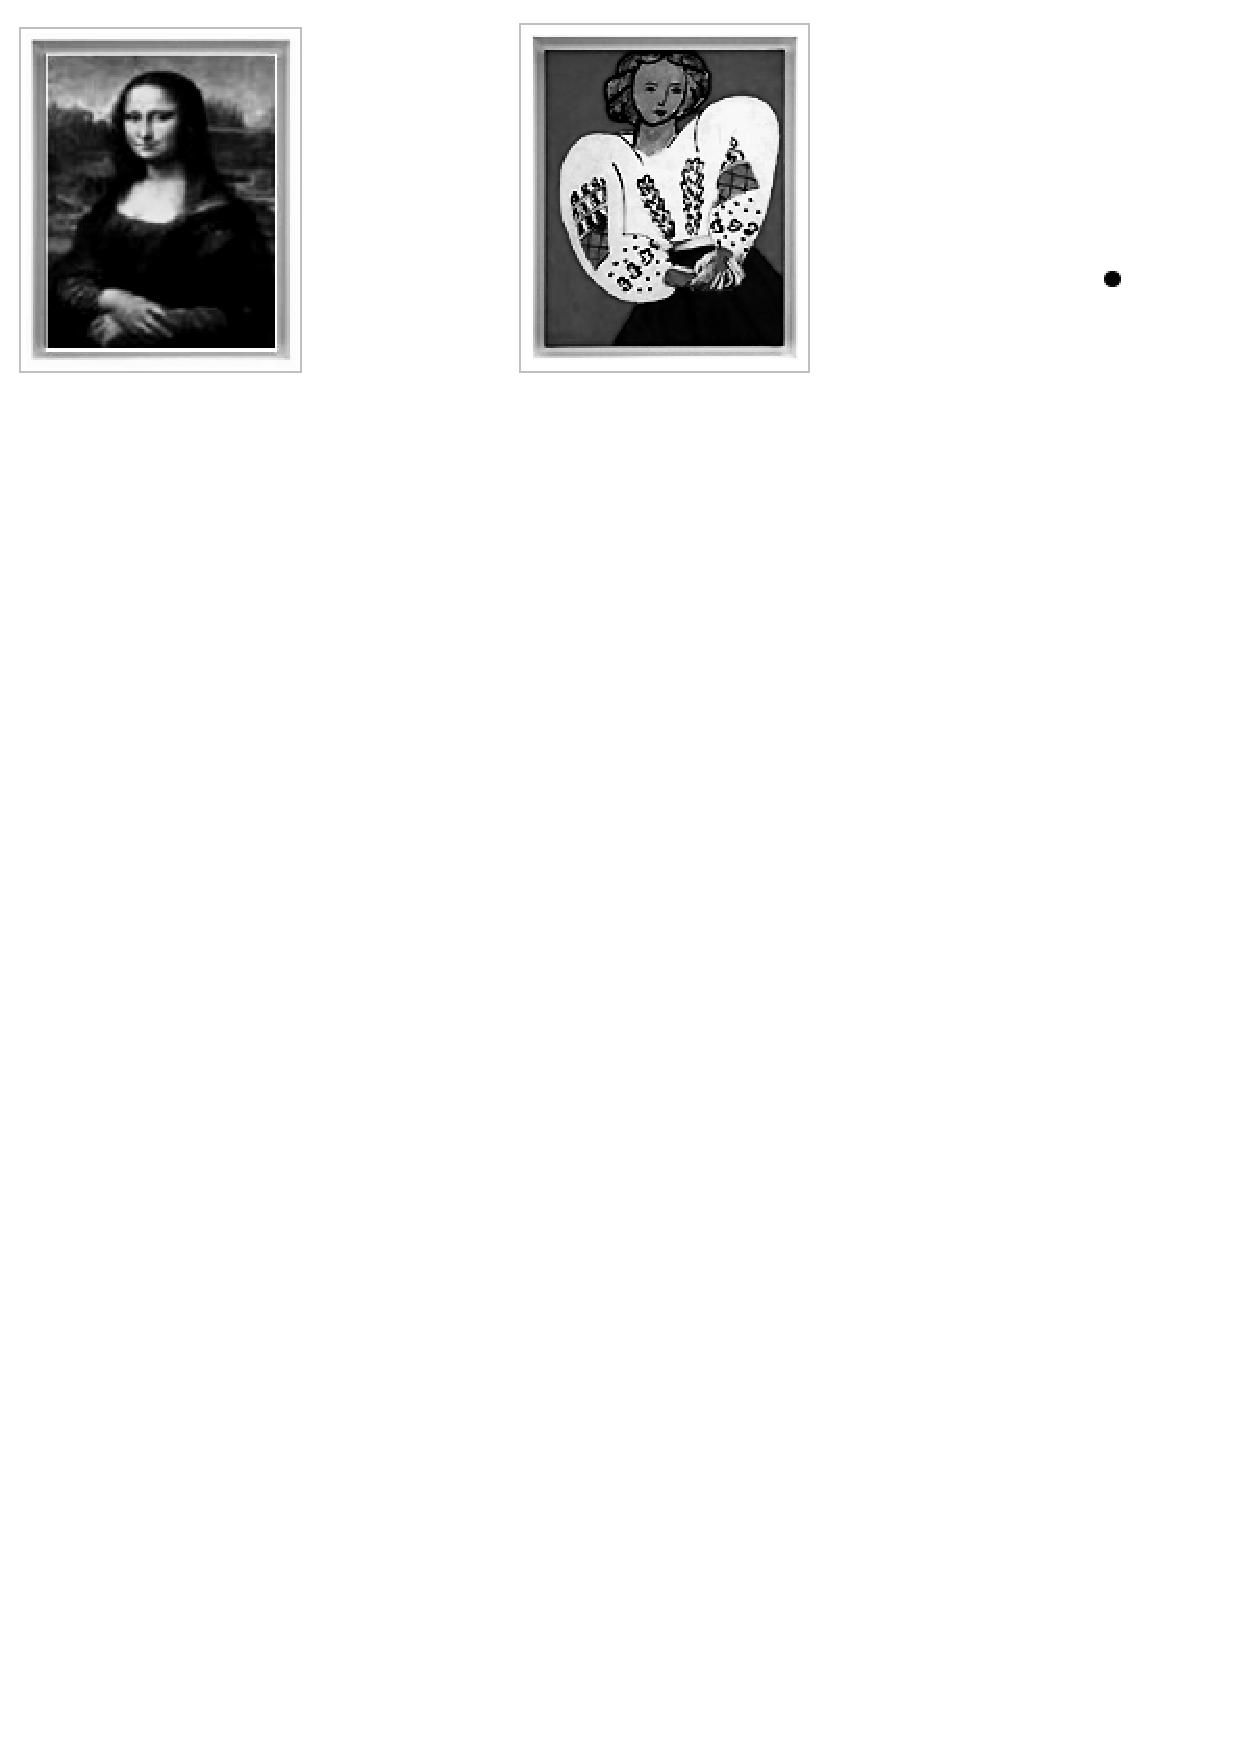
\includegraphics[scale=.6]{tableaux.jpg}
    \end{center}
    \caption{Échanger les deux tableaux en utilisant le clou libre}
    \label{fig:ex_onto}
\end{figure}

\begin{correction}
\begin{verbatim}
/* tableau 1 (clou 1) -> clou 3 */
/* tableau 2 (clou 2) -> clou 1 */
/* tableau 1 (clou 3) -> clou 2 */
\end{verbatim}
\end{correction}

\subsection{Échange des valeurs de deux variables en C}

\begin{enumerate}
\item 
  Écrire un programme C qui déclare et initialise deux variables
  entières \C{x} et \C{y} et effectue la permutation de ces deux
  valeurs. Commencer par écrire un algorithme, à l'aide de phrases telles que << Copier la valeur de la variable ... dans la variable ...>>, en vous inspirant de la question précédente.
\begin{correction}
L'agorithme doit être utilisé pour structurer le code. On ne donne pas ici de valeur à $x$ et $y$, mais n'hésitez pas à en donner (par initialisation par exemple). 

{\small
\listinginput{1}{echange.c}
}
\end{correction}

\item Traduire ce programme C en un programme amil. On supposera que les deux variables sont stockées aux adresses \C{10} et \C{11}.
  \begin{correction}
    À nouveau, l'algorithme est à utiliser en commentaires pour
      structurer le code.
\begin{verbatim}
# copie de la case d'adresse 10 dans une case auxillaire (12)
 1 lecture 10 r0
 2 ecriture r0 12
# copie de la case d'adresse 11 à l'adresse 10
 3 lecture 11 r0
 4 ecriture r0 10
# copie de la case auxillaire à l'adresse 11
 5 lecture 12 r0
 6 ecriture r0 11
 7 stop
 9 
10 4
11 5
12 ?
\end{verbatim}
  \end{correction}
%\item Exécuter ces programmes sur un exemple (faire les traces).
\begin{correction}
 \begin{figure}
  \centering
  \begin{tabular}[c]{|c|c|c|c|c|c|c|}
\hline
Cycles & CP & instruction & r0& 10& 11& 12\\ \hline
INIT & 1 & & ? & 4
 & 5
 & ?
 \\ \hline1 & 2 & \commentaire{Lecture de la donnée d'adresse 10 dans le registre 0
} lecture 10 r0
 & 4 & & & \\ \hline
2 & 3 & \commentaire{Écriture du registre 0 à l'adresse 12
} ecriture r0 12
 & & & & 4
 \\ \hline
3 & 4 & \commentaire{Lecture de la donnée d'adresse 11 dans le registre 0
} lecture 11 r0
 & 5 & & & \\ \hline
4 & 5 & \commentaire{Écriture du registre 0 à l'adresse 10
} ecriture r0 10
 & & 5
 & & \\ \hline
5 & 6 & \commentaire{Lecture de la donnée d'adresse 12 dans le registre 0
} lecture 12 r0
 & 4 & & & \\ \hline
6 & 7 & \commentaire{Écriture du registre 0 à l'adresse 11
} ecriture r0 11
 & & & 4
 & \\ \hline
7 & 8 & \commentaire{Fin du processus.
} stop
 & & & & \\ \hline
\end{tabular}
  \caption{Simulation de l'échange de deux valeurs en mémoire (4 et 5)}
  \label{simsw1}
\end{figure}
  \end{correction}
\item (Facultatif). Donner d'autres solutions en assembleur à ce problème (la permutation des contenus des adresses \C{10} et \C{11}).
  \begin{correction}
Par exemple : 
\begin{verbatim}
# copie de la case d'adresse 10 dans un registre pour sauvegarde
1    lecture 10 r1
# copie de la case d'adresse 11 à l'adresse 10
2    lecture 11 r0
3    ecriture r0 10
# copie de a dans registre de sauvegarde à l'adresse 11
4    ecriture r1 11
5    stop
\end{verbatim}
\begin{figure}
  \centering
  \begin{tabular}[c]{|c|c|c|c|c|c|c|}
\hline
Cycles & CP & instruction & r0& r1& 10& 11\\ \hline
INIT & 1 & & ? & ? & 4
 & 5
 \\ \hline1 & 2 & \commentaire{Lecture de la donnée d'adresse 10 dans le registre 1
} lecture 10 r1
 & & 4 & & \\ \hline
2 & 3 & \commentaire{Lecture de la donnée d'adresse 11 dans le registre 0
} lecture 11 r0
 & 5 & & & \\ \hline
3 & 4 & \commentaire{Écriture du registre 0 à l'adresse 10
} ecriture r0 10
 & & & 5
 & \\ \hline
4 & 5 & \commentaire{Écriture du registre 1 à l'adresse 11
} ecriture r1 11
 & & & & 4
 \\ \hline
5 & 6 & \commentaire{Fin du processus.
} stop
 & & & & \\ \hline
\end{tabular}
  \caption{Simulation de l'échange de deux valeurs en mémoire (4 et 5), avec un second registre}
  \label{simsw2}
\end{figure}
  \end{correction}

\item (Facultatif). Mêmes questions que précédemment mais pour faire une permutation
  circulaire de 3 valeurs.

  \begin{correction}    


{\small
\listinginput{1}{echange3.c}
}

Sans le second registre (traduction) :
\begin{verbatim}
lecture 10 r0  
ecriture r0 13 
lecture 11 r0  
ecriture r0 10 
lecture 12 r0  
ecriture r0 11 
lecture 13 r0  
ecriture r0 12 
stop
\end{verbatim}
Avec le second registre :
\begin{verbatim}
lecture 10 r1  
lecture 11 r0  
ecriture r0 10 
lecture 12 r0  
ecriture r0 11 
ecriture r1 12 
stop
\end{verbatim}
\end{correction}
\end{enumerate}


\begin{correction}
  Note aux chargés de TD.
  \begin{itemize}
  \item En cours, ils ont vu les variables impératives et
    le if. Leur sémantique a été donnée par leur traduction en langage
    amil.
  \item Ils doivent savoir resoudre/reproduire les exos marqués exercices types et faire leur trace sur un exemple quelconque.
  \item On applique la procédure de résolution :
    \begin{itemize}
    \item on se donne des exemples
    \item on trouve un algorithme en francais
    \item on traduit l'algorithme en C, en s'aidant de commentaires
    \item on teste sur les exemples 
    \end{itemize}
  \item Le code de la fonction main vide en C a ete présenté rapidement, commenté avec les differents points qu'ils vont voir au semestre. Il est long et peut etre raccourci mais il faut s'assurer qu'ils sachent écrire ce genre de préambule du C avant d'écrire leurs programmes.
  \item Le code leur est toujours donné avec les commentaires, en suivant scrupuleusement l'indentation choisie. Ils doivent bien comprendre que le code et les commentaires sont indissociables. N'hesitez pas a ajouter des commentaires en fonction des difficultés rencontrées dans votre groupe.
  \end{itemize}
\end{correction}

%\subsection{Pour essayer en TP}

\section{Exécution conditionnelle d'instructions :  \emph{if}}
Les programmes suivants réalisent des affichages, pour cela nous
utiliserons la fonction \C{printf}, disponible après avoir inséré
\verb|#include <stdio.h>| en début de programme (ligne~3 dans le
programme figure~\ref{fig:programmes}). 

Testez vos programmes sur
machine (avec l'aide de votre enseignant).

\subsection{Majeur ou mineur ?}

Soit la variable \verb|age|, contenant l'âge d'une personne. Écrire un
programme qui affiche si cette personne est majeure ou
mineure. Indication : \verb|printf("Vous êtes majeur !\n");| affiche
\C{Vous êtes majeur !} et un saut de ligne.

\begin{correction}
\begin{verbatim}
algorithme :
si age >= 18 alors 
  affiche majeur
sinon 
  affiche mineur
\end{verbatim}
\begin{listing}{1}
/* Declaration de fonctionnalites supplementaires */
#include <stdlib.h> /* EXIT_SUCCESS */
#include <stdio.h> /* printf */

/* Declaration des constantes et types utilisateurs */

/* Declaration des fonctions utilisateurs */

/* Fonction principale */
int main()
{
    /* Declaration et initialisation des variables */
    int age = 16; /* age de la personne */

    if(age >= 18) /* majeur */
    {
	/* affiche majeur */
	printf("Vous êtes majeur.\n");
    }
    else /* mineur (age < 18) */
    {
	/* affiche mineur */
	printf("Vous êtes mineur.\n");
    }
    
    /* valeur fonction */
    return EXIT_SUCCESS; /* renvoie OK */
}

/*Definitions des fonctions utilisateurs */
\end{listing}
\end{correction}

\subsection{Exercice type :  le minimum de 3 valeurs}

Soient 3 variables \verb|a|, \verb|b|, \verb|c|, initialisées à des
valeurs quelconques. Écrire un programme qui calcule et affiche à
l'écran le minimum des 3 valeurs.  

Indication : si \C{x} est une variable contenant l'entier 42,
\verb|printf("Solution : %d\n", x);| affichera \C{Solution : 42} et
un saut de ligne.

\begin{correction}
\begin{verbatim}
algorithme :
soit min = a /* valeur par defaut */
si b < min /* b plus petit que min courant */
  /* b est le min courant */
  min = b
/* min contient min(a,b) */
si c < min /* c plus petit que min courant */
  /* c est le min courant */
  min = c
/* min contient min(min(a,b),c) = min(a,b,c) */
affiche min
\end{verbatim}
\begin{listing}{1}
\end{listing}
\end{correction}

\subsection{Exercice type : Dans une seconde, il sera exactement\ldots}

Écrire un programme qui, étant donnée une heure représentée
sous la forme de trois variables : une pour les heures, \verb|h|, une pour
les minutes,
\verb|m| et une pour les secondes, \verb|s|, affiche l'heure qu'il sera une
seconde plus tard. Il faudra envisager tous les
cas possibles pour le changement d'heure. Deux exemples de sortie sont~:

\begin{verbatim}
L'heure actuelle est : 23h12m12s
Dans une seconde, il sera exactement : 23h12m13s

L'heure actuelle est : 23h59m59s
Dans une seconde, il sera exactement : 00h00m00s
\end{verbatim}

Pour l'affichage :  
\verb|printf("L'heure actuelle est : %dh%dm%ds\n", h, m, s);|.

\begin{correction}
Mieux (hors programme) :
  \verb|printf("L'heure actuelle est : %02dh%02dm%02ds\n", h, m, s);|.
\end{correction}

\begin{correction}
\begin{verbatim}
algo :
- affiche l'heure actuelle
- ajoute une seconde
- si tour du cadran des secondes alors
    - remise a 0 des secondes
    - il est une minute de plus
    - si tour du cadran des minutes alors
        - remise a 0 des minutes
        - il est une heure de plus
        - si tour du cadran des heures alors
    	    - remise a zero des heures
- affiche la nouvelle heure
\end{verbatim}
  \begin{listing}{1}
/* Declaration de fonctionnalites supplementaires */
#include <stdlib.h> /* EXIT_SUCCESS */
#include <stdio.h> /* printf */

/* Declaration des constantes et types utilisateurs */

/* Declaration des fonctions utilisateurs */

/* Fonction principale */
int main()
{
    /* soient 23h59m59s */
    int h = 23;
    int m = 59;
    int s = 59;

    /* affiche l'heure actuelle */
    printf("L'heure actuelle est : %dh%dm%ds\n",h,m,s);

    /* une seconde de plus */
    s = s + 1;

    if(s == 60) /* tour du cadran des secondes */
    {
	/* remise a 0 */
	s = 0;

	/* une minute de plus */
	m = m + 1;

	if(m == 60) /* tour du cadran des minutes */
	{
	    /* remise a 0 */
	    m = 0;

	    /* une heure de plus */
	    h = h + 1;

	    if(h == 24) /* tour du cadran des heures */
	    {
		/* remise a zero */
		h = 0;
	    }
	}
    }
    /* h,m,s contiennent l'heure une seconde plus tard */

    /* affiche l'heure */
    printf("Dans une seconde, il sera exactement : %dh%dm%ds\n",h,m,s);

    /* valeur fonction */
    return EXIT_SUCCESS;
}

/* Definitions des fonctions utilisateurs */
  \end{listing}
\end{correction}


%%% Local Variables: 
%%% mode: latex
%%% TeX-master: "td1"
%%% End: 
